\documentclass[a4paper,12pt]{article} 
\usepackage[margin=1in]{geometry}
\usepackage[utf8]{inputenc}
\usepackage[english]{babel}
\usepackage{fancyhdr}
\usepackage{mathtools}
\usepackage{float}
\usepackage{hyperref}
\usepackage[toc,page]{appendix}
\usepackage{listings}
\lstset{
basicstyle=\small\ttfamily,
columns=flexible,
breaklines=true
}

\hypersetup{pdfborder=0 0 0}

\pagestyle{fancy}
\fancyhf{}
\rfoot{Page \thepage}


\begin{document}

\begin{titlepage}
   \begin{center}
       \vspace*{1cm}
 
       \textbf{CAB320 Artificial Intelligence - Semester 1 2022}
 
       \vspace{0.5cm}
        \LARGE{Development of a Solver for Sokoban Puzzels}
 
       \vspace{1.5cm}

       \vfill
       
       \vspace{0.8cm}
       \normalsize
 	   Written in \LaTeX \\
       
\includegraphics[width=0.4\textwidth]{QUT.jpg}

       \large
       \textbf{Jake Burrell}\\
       \textbf{n9712291}
       \textbf{Edward Duong}\\
       \textbf{n10113266}
       \textbf{Pravindkumaran Baskaran}\\
       \textbf{n9795651}

       \vspace{1.5cm}
 
       \normalsize
       Faculty of Science \\
       Queensland University of Technology\\
       Australia\\ 
   \end{center}
\end{titlepage}

%\tableofcontents

\section{Solver}
% Briefly discuss how A* search algorithm has been implemented in order to solve the problem 
The sokoban puzzle can be modeled as a graph structure wherein each state represents that of the position of a player and the position of each of the boxes. The initial state will act as the first starting node in the graph. From the initial state, with every legal movement, it will spawn a maximum of 4 states corresponding to 4 moves left, right, up and down that the player can go. These actions then make each of the connected nodes that can be expanded from the initial state. The cost of making any one of these actions can be viewed as a weighted and directed edge between these two nodes in the graph. Using this representation the goal state or solution node is the state in which all the boxes are on targets. It is for this reason that the A* a graph search algorithm can be used in order to find this goal state. Using this alogithm each generated state will have its own evaluation value (depended on the heuristic function) and is sorted into a priority queue so that the A* algorithm can get from the queue to browse to reach the target state quickly.

\subsection{State Representation}
% Used a class to represent the state representation
% Container for both two properties worker and boxes both of which were tuples in the form ((x,y) 
% Overrode methods such to make sate representation hashable to allow it to be stored in a the frontier set
% Overrode less than method to allow it co be compared in the best first search
The state representation chosen was that of a State class containing two tuples one to  represent the position of the worker and one nested tuple to represent the positions of each of the boxes. The worker's position was stored in the form (x,y), x being the horizontal axis and y being the vertical with the origin (0,0) in the top left of the map. Similarly the tuple components representing individual boxes stored within the box's tuple were also stored as such. These particular values were chosen as the state representation because with each move or action made within the sokoban puzzle these were the only values with a propensity to change and thus they are dynamic. In order to make this particular state representation usable within the SokobanPuzzle class a number of methods had to be overridden. These such methods include that of \textunderscore eq \textunderscore and \textunderscore lt\textunderscore method used to calculate equalities and comparisons with State objects. Both of which are used by the best\textunderscore first\textunderscore graph\textunderscore search algorithm. Additionally the methods \textunderscore key\textunderscore  and \textunderscore hash\textunderscore  were implemented in order to allow state instances to be hashable as to allow them to be added into sets, such as in the frontier set in the best\textunderscore first\textunderscore graph\textunderscore search again. Note, this best\textunderscore first\textunderscore graph\textunderscore search function is utilized to implement A* graph search algorithm simply by passing it the heuristic to be used in its priority queue.
 

\begin{lstlisting}
State: the current positions of a player and the boxes.
Initial State: The start positions of player and the boxes depended on the map
Goal State: The state that all boxes are on the target places
Legal move: Assume that the position of player (x,y) and the top left corner is (0,0)
Up: (x,y) => (x,y-1)
+ Neither box nor wall at the position (x, y-1) 
+ If there is a box at the position (x, y-1), we have to ensure that neither box nor wall at the position (x, y-2)

Down: (x,y) => (x,y+1)
+ Neither box nor wall at the position (x, y+1) 
+ If there is a box at the position (x, y+1), we have to ensure that neither box nor wall at the position (x, y+2)

Left: (x,y) => (x-1,y)
+ Neither box nor wall at the position (x-1, y) 
+ If there is a box at the position (x -1, y), we have to ensure that neither box nor wall at the position (x - 2, y)

Right: (x,y) => (x + 1, y)
+ Neither box nor wall at the position (x+1, y) 
+ If there is a box at the position (x+1, y), we have to ensure that neither box nor wall at the position (x+2, y)
 
\end{lstlisting}

\subsection{Heuristic}
% Explain what the heuristic is calculating and how it is valid for the problem
% Prove that it is admissible
% Potentially prove that it is consistent otherwise demonstrate its consistent by discussing test of consistency
% Potentially include illustration demonstrating what its calculating compared to actual cost

In the A* search algorithm the purpose of the heuristic is to provide a rough but fast estimate on the weighted distance from the current state to the goal state. It can be demonstrated that for any A* tree search, provided the heuristic is admissible it will always produce an optimal path. For a heuristic to be admissible it must at no state make an overestimate to the true optimal cost of reaching the goal state. In A* graph search algorithm however, which is the one implemented for this problem, the heuristic must have an additional trait. This trait is that of consistency and implies that the difference in the heuristic evaluated at any node ‘A’ and at any one child node of ‘A’, must always be less than or equal to the actual cost between those two nodes. Note that for this problem, the sokoban puzzle, a node represents a particular state and a child node would be any node representing a state within one action or movement from that state.
\\

The Heuristic chosen to use for the solution we implemented simply calculates the Manhattan distance to the closest box from the workers position. Then it calculates the weight associated with the worker moving each box to the nearest target. This is done by calculating the manhattan distance to each target from each box multiplied by the weight of the worker plus the box weight. The shortest of these weighted distances for each box is then added together. Additionally the manhattan distance of the worker to each box is calculated and the shortest of these distances is also added to the aforementioned distances. The resultant sum gives the heuristic value at any state in the sokoban puzzle.
\\

First the heuristic that was used is demonstrably admissible because in all situations the actual cost of reaching a goal state must be equal to or more than the heuristic. This is because to reach the goal state the worker must first, in the best case travers to each position between it and a target. Doing so would result in a cost equal to the manhattan distance to that box. Next the worker must then at least in the best case traverse each square between each box and that box's closest target. This would result in a cost equal to the manhattan distance between that box and the target, for the cost incurred by the worker. Plus it also incurred a cost from the movement of the box equal to this same Manhattan distance calculation multiplied by that box's weight. Since the heuristic is calculated from these same calculations it must in all cases be admissible. 
\\

Similarly the heuristic is consistent because in all cases if the worker is simply moving itself in a single action the cost of this move is only one. Transversely the difference in the heuristic between these two states can only be decreased by one. This is because if the worker is only moving one position the distance to the closest target can only diminish by one. In this situation the box to target distances will not change. In cases where the worker is moving a box in a single action, the cost will be equal to that of one plus the weight of the box. In such a state transition the difference in the heuristic between these two states can never be more than the aforementioned cost. This is because in such a situation the distance to the closet box will always be one, representing the cost incurred by the worker. Additionally the distance from each box to their closest target can never be diminished by more than one. For this reason in all cases the heuristic must be consistent.


\subsection{Other Classes and Methods}
% Brief outline how puzzle class interacts with search class and utilizes taboo cells
%\subsubsection{SokobanPuzzle}
% Explain SokobanPuzzle class:
    % Discuss initial parameters noting that taboo\textunderscore cells is an optional parameter
    % Discuss functions: (Uses method docstring maybe touch on implementation )
        % result
        % actions
        % goal\textunderscore test
        % path\textunderscore cost
        % box\textunderscore movable mention how it checks taboo cells if they exist 

    \begin{figure}[H]
        \centering
        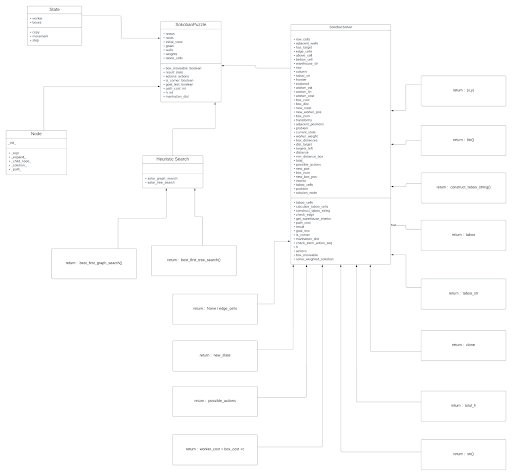
\includegraphics[width=18cm]{uml.png}
        \caption{UML Class diagram}
        \label{fig:svm_conf}
    \end{figure}
\subsubsection{Taboo Cells}
% Explain taboo cells function:
    % Modified Breadth first search algorithm to determine interior cells
    % is\textunderscore corner method applied to all interior cells using transforms to calculate adjacent cells and thus determine corners
    % Edges were found from corners and checked if entire edge was along a wall using check\textunderscore edge 
    % Corners and edges made taboo cells
% Potentially add diagram explaining what taboo cells are 

Taboo cells are cells which are part of the internal structure of the game, if an object gets pushed to a taboo cell, the space around it becomes limited so it prevents the player from moving the box from current state to a goal state. To determine taboo cells there are two rules. First, if a cell is corner and not a target then it is a taboo cell because the worker cannot move behind the box to move it off the walls. The next situation is when the cells between two corners along a wall have no targets. In such a case the box cannot be moved off this wall and if there are no targets on this wall it can never reach a target.

\section{Testing}
% Discuss how each tests was preformed on all major methods to validate their output
% Mention they we based off tests found in sanity\textunderscore check
% Discuss how solver tests checked timings and checked against provided solutions in the FAQ
% Method how we used a mixture of black box and white box testing
    % I.E Some tests were done prior to completing methods additional tests added after completion
% Might add addition tests
% Potentially add table showing what was tested and too what degree 

To ensure the sokoban game solver functions correctly a number of tests were created to ensure its accuracy. The development of these tests were based on the included sanity\textunderscore check file. Each of the vital methods involved with deploying the sokoban solver were tested using a mixture of black and white box testing. First of all in order to establish the taboo cells the interior of the warehouse had to be established. In order to do so a method was developed and tested to do so. Next a test was made to check for corner membership and a method was implemented meeting these tests. The check edge method was also developed and then tested with the test\textunderscore check\textunderscore edge method. Once that was done and a number of tests were created to test taboo cells and actions. The results methods and check elem action sequence methods were also tested to ensure their integrity. Note, no mocks or stubs were utilized in this particular test so these tests did require the correct implementation of results and actions. Doing so did undermine the independence of this particular test. This was done for convenience however, allowing less rigorous tests to be required for these methods. Check element sequence method as itself was not vital to the solver and functioned itself as a reasonably comprehensive test of these two methods. After this the heuristic was developed and tested to check it for admissibility and consistency. Both of which were done with two separate testing methods utilizing multiple separate tests. For the test\textunderscore h\textunderscore consistency each consecutive state in the solution for warehouse 147 were checked to ensure they met the consistency requirement. Lastly the solver was tested and checked against a number of solutions provided in the FAQ. Timers were also implemented allowing the completion times of these solutions to be compared. 

\section{Performance and Limitations}
% Discuss what problems it can complete and how long it takes
% Generalized explaining what sort of problems it preforms quickly on and which ones it does not
% Mention for example how it takes a long time to confirm warehouse 5n is impossible
% Discuss why some examples seem to be significantly slower then the ones found in the FAQ
    % Reasons for this most likely due to using a class for the state representation as opposed to a tuple of tuples
    % Mention that class instantiation and deconstruction takes additional time as it must instantiate the class object and its nested classes, in the form of the worker and box tuples
    % Not maybe that this does make the code look cleaner and more readable
% Use table too display times for each problem

After tested the functional of Sokoban solver, the performance shows that using the A* rather than another algorithm to solve the Sokoban game is most effective on solving time. It always produces an optimal solution because it will expand the most optimal nodes first, based on the heuristic. This means that the solution solves the puzzles more easily and faster than a standard breadth first graph search. Additionally, as the movement constraint of the game, the player can only move horizontally or vertically and it all costs 1 for every move. The use of Manhattan in order to create a heuristic function produces a consistent result used for priority queue. As a result, the A* algorithms will always create a sufficient and efficient solution. The result of the solver was mostly exemplary. However, using a class for the state representation as opposed to a tuple of tuples may cause some examples to be significantly slower than normal(Figure 1). Instantiation and deconstruction takes additional time as it must instantiate the class object and its nested classes, in the form of the worker and box tuples. Use of a more streamlined state representation would most likely resulted in faster solution times. Despite this our solution had reasonable performance, the solver also shows few limitations. The use of A* search is flexible but will have to use a lot of memory to save the passed states. 

\begin{figure}[h]
    \centering
    \begin{tabular}{|l|l|l|l|}
    \hline
    \multicolumn{1}{|c|}{Warehouse} & \multicolumn{1}{c|}{Difficult level} & \multicolumn{1}{c|}{Time solving(s)} & \multicolumn{1}{c|}{Costs} \\ \hline
    41                              & Easy                                 & 0.196                                & 50                         \\ \hline
    15                              & Easy                                 & 0.052                                & 37                         \\ \hline
    5n                              & Impossible                           & 31.730                               & None                       \\ \hline
    8a                              & Medium                               & 4.285                                & 431                        \\ \hline
    03\_impossible                  & Imposible                            & 0.064                                & None                       \\ \hline
    147                             & Medium Difficult                     & 8228.731                             & 521                        \\ \hline
    \end{tabular}
    \caption{Solution Performance}
\end{figure}



\end{document}